\documentclass{article}
\usepackage{amsmath}
\usepackage{verbatim}
\usepackage[margin=1in]{geometry}
\setlength\parindent{0pt}
\usepackage{color}
\usepackage{graphicx}
\usepackage{hyperref}
% \usepackage{subcaption}
%\usepackage{tabularx}
%\usepackage{float}

\begin{document}


\begin{center}
\Huge{\textsc{Homework Five Report}} 

\Large\textsc{CMPS242 - Fall 2015}\\

\large{Andrei Ignat  \hfill Sabina Tomkins \hfill Guangyu Wang} 
\end{center}

%fix the title

\section{Intro}
The data was obtained from the Kaggle competition website. We preprocessed the data by selecting certain features and discarding other features, due to reasons mentioned in Section~\ref{sec:preproc}. For classification, we used a number of routines from the \texttt{python}-based package, \texttt{scikit-learn}. These classifiers and the reasons we chose them are described in Section~\ref{sec:envi}. The results are presented in Section~\ref{sec:res}, with the corresponding analysis in Section~\ref{sec:anal}

\section{Data Preprocessing}
\label{sec:preproc}
Due to a high number of missing values, the data is difficult to process \textit{as-is}. After running a correlation check using the built-in \texttt{pandas} Kendal-Tau correlation coefficient, we decided to keep the features named \texttt{Pclass}, \texttt{Fare}, \texttt{Gender} and to combine the features \texttt{Age} and \texttt{Parch} into a single feature \texttt{Page} using the formula

\[
\mathtt{Page} = \mathtt{Parch} \times \mathtt{Age}  
\]

The reason for building this new variable is given by the relatively high importance of the \texttt{Parch} variable. Since, there is a high number of missing values in the \texttt{Age} feature, and we did not want to replace these with the average age, we decided on integrating the existing \texttt{Age} values into \texttt{Parch}. Wherever there was a missing value on either side, the value of the \texttt{Parch} feature was simply set to 0. 

The remaining features were simply dropped due to their low correlation coefficients.

\section{Environment}
\label{sec:envi}
We used \texttt{python} exclusively, and in particular we used \texttt{scikit-learn} for all classifiers. The classifiers we used, along with the motivation behind each of them, are:

\begin{itemize}
\item \textbf{Support Vector Machine} - a classical and almost benchmark test for a classification problem. In this case, the separating margin indicates the distance of each individual from the \textit{survival line}
\item \textbf{Logistic Regression} - another classical method for classification problems, the logistic regression was chosen in order to account for a higher more relaxed model than the SVM. In this case, the variables are allowed to influence the survival rate in a probabilistic manner.
\item \textbf{K Nearest Neighbors} - yet another classical classification routine, the KNN classifier was tuned for different numbers of neighbors and trained on the dataset.
\item \textbf{Decision Trees} - were used due to their inherent simplicity. We did not expect perfect results from them though and that's why we bootstrapped them to Random Forests and Adaptive Boosting.
\item \textbf{Random Forest} - Random forests were used in an attempt to improve the accuracy of a decision tree classifier. 
\item \textbf{AdaBoost} - Adaptive boosting was used to improve the performance of the decision tree classifier in an attempt to get a higher accuracy.
\end{itemize}


\section{Results}
\label{sec:res}
\subsection{Individual Classifiers}
Each of the following classifiers we tried on its own, and tried to tune the parameters for. When we combined classifiers we therefore used the best parameters found in the parameter tuning process. The classifiers we used are: Support Vector Machine, Logistic Regression, AdaBoost, Random Forest, Decision Trees, and K Nearest Neighbors. We chose these classifiers as they have been covered in class, \\

[insert a reason for each one why it may do ok on this dataset]  \\

Accuracy was used as the metric with which to compare classifiers. To see the results from the parameter tuning process please see the Appendix. Both in the parameter tuning, and in the final results below, we used 5-Fold cross validation. However in the ensemble we held out 40\% of the training set for validation.\\

\begin{tabular}{|c|c|c|c|c|c|c|}
\hline
& SVM & Decision Trees & KNN & Random Forest & Logistic Regression & AdaBoost   \\
\hline
Accuracy & SVM & Decision Trees & KNN & Random Forest & Logistic Regression & AdaBoost   \\

\hline
\end{tabular}\\

\subsection{Combined Classifiers}


\section{Analysis}
\label{sec:anal}

\section{Appendix}
\graphicspath{../}

 \begin{figure}[h!]
 \centering
  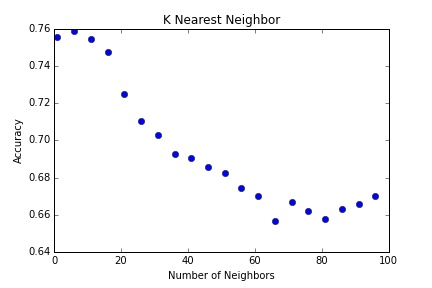
\includegraphics[width=0.5\textwidth]{NearestNeighbor.jpg}
 \caption{Tuning number of neighbors nearest neighbor}
 \end{figure}

 \begin{figure}[h!]
 \centering
  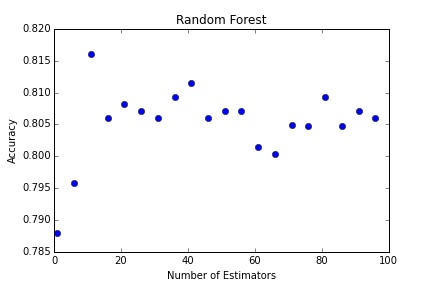
\includegraphics[width=0.5\textwidth]{RandomForest.jpg}
 \caption{Tuning number of estimators, Random Forest}
 \end{figure}
 
 


\bibliography{proposal_biblio}
\bibliographystyle{plain}

\end{document}
